%!TEX root = ../../lod-group1.tex
\subsection{Movie Ontology}
\label{subsec_method_ontology}

As described in the previous section, different data sources, each having their own data format, were used in the system \emph{Match Forrest, Match!}.
To create a unified dataset and therefore enable simple querying over all data, an ontology for movies was defined.

This ontology covers movie resources as well as resources, which belong to a movie, such as awards.
In general, the defined ontology is based on the DBpedia ontology.
Where possible, classes and properties where used from DBpedia and Freebase (in this order).
If no were present, new classes or properties were defined.

In the following, the defined entities used in the system are listed with their corresponding RDF classes in Table~\ref{tab_entities}.

\begin{table}[ht]
	\begin{center}
	\begin{tabular}{ll}
		\textbf{Entity} & \textbf{RDF class} \\ \hline
		Movie & dbpedia-owl:Film \\
		Award & dbpedia-owl:Award \\
		MoviePerson & dbpedia-owl:Person \\
		Character & freebase:film/performance \\
		MovieCharacter & lod:MovieCharacter \\
		Aka (also known as) & lod:Aka \\
		ReleaseInfo & lod:ReleaseInfo \\
	\end{tabular}
	\end{center}
	\caption{Entities with their corresponding RDF classes.}
	\label{tab_entities}
\end{table}

Relations between these resources and their pattern for the unique identifiers are shown in Figure~\ref{fig_ontology}.
The prefix \textit{lod} was newly defined for this project.

\begin{figure}[h!]
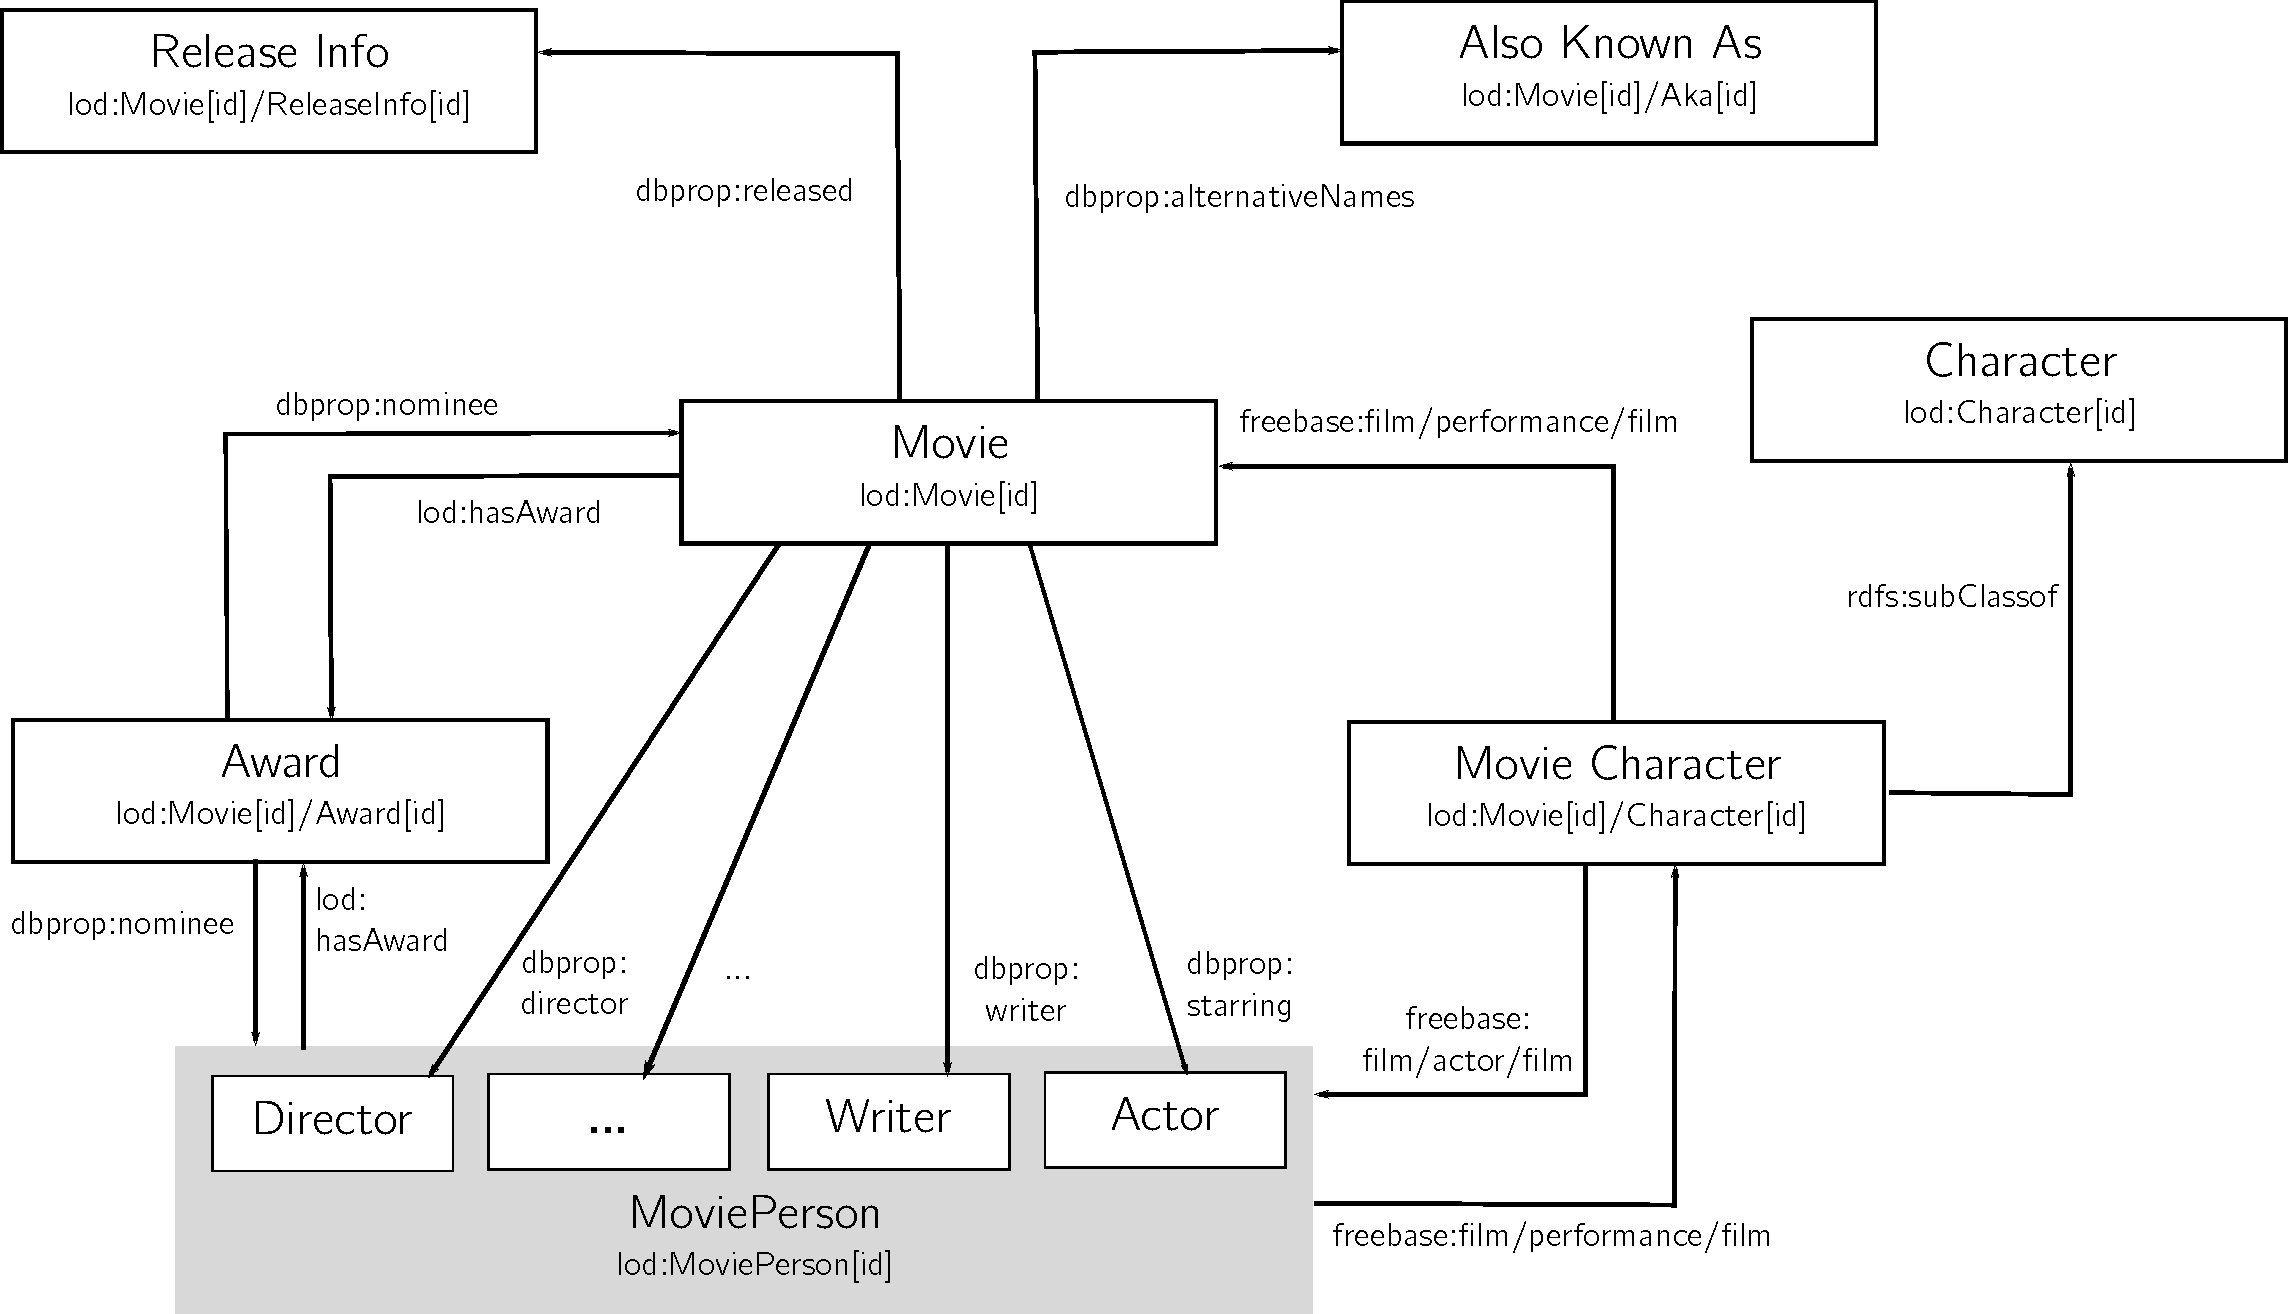
\includegraphics[width=\textwidth]{images/ontology.pdf}
\caption{Entities of the movie ontology and their relations and patterns for the unique identifiers.}
\label{fig_ontology}
\end{figure}

A MoviePerson can have multiple sub-types of \textit{dbpedia-owl:Person}, depending on the jobs the person had on any movies they worked on.
As shown in Figure~\ref{fig_ontology} a distinction between these jobs (e.g. director, writer, producer) was made.
For example, a person who is a director in one movie and an actor in another movie would have the additional classes \textit{dbpedia-owl:Actor} and \textit{dbpedia-owl:Director}.

A problem, which occured when defining our ontology, was the entity Character.
In the initial definition, there was just one character class, which was connected to the corresponding movie and actor.
The actor also had a connection to the character.
The unique identifier of the character was build from the character's name.

Thus, a character, which exists in multiple movies (e.g. ``cleaning lady''), would be one resource connected to each actor, who had ever portrayed this character.
The character also had a list of movies, which it occured in.
That way, one could not say, which actors played the character in a certain movie.
One such case is an actor, who played a certain character in an old movie, but also appears in the movie's newer remake.
In the remake, they might play a different character while another actor plays their original character.
An example for this is the movie ``Starsky \& Hutch'' (2004), which is a remake of the 1970s television series with the same name.
In the movie, both actors, which originally portrayed Starsky and Hutch get a cameo appearance alongside the new cast for their old characters.
With the old approach, the system could not know who played the Starsky character in the remake, because all actors who ever played the character are listed.

Therefore, an additional class of MovieCharacter was introduced in the final ontology.
This resource is only connected to one movie and all actors, who played that character in that movie.
The unique identifier of the MovieCharacter is build from the unique identifier of the movie and the character.
The MovieCharacter is a subclass of Character, which describes the general character.
This means, that the unique identifier of the MovieCharacter in the ``Starsky \& Hutch'' example is ``Starsky/Starsky\&Hutch1970'' and the identifier of Character is ``Starsky''.